\documentclass[12pt]{article}
 \usepackage[margin=1in]{geometry} 
\usepackage{amsmath,amsthm,amssymb,amsfonts}
\usepackage{graphics} 
\usepackage[dvipdfmx]{graphicx}

\newcommand{\N}{\mathbb{N}}
\newcommand{\Z}{\mathbb{Z}}
 
\newenvironment{problem}[2][Problem]{\begin{trivlist}
\item[\hskip \labelsep {\bfseries #1}\hskip \labelsep {\bfseries #2.}]}{\end{trivlist}}
%If you want to title your bold things something different just make another thing exactly like this but replace "problem" with the name of the thing you want, like theorem or lemma or whatever
 
\begin{document}
 
%\renewcommand{\qedsymbol}{\filledbox}
%Good resources for looking up how to do stuff:
%Binary operators: http://www.access2science.com/latex/Binary.html
%General help: http://en.wikibooks.org/wiki/LaTeX/Mathematics
%Or just google stuff
 
\title{HW 1}
\author{Motoaki Takahashi}
\maketitle
\section{Question 1}

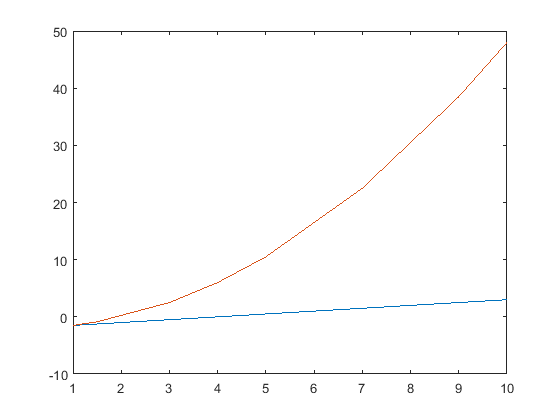
\includegraphics{q1.png}\par
$Y1$ and $Y2$ are shown above, where the blue line is $Y1$ and the red curve is $Y2$.

\section{Question 2}
The $200\times1$ vector that contains evenly-spaced numbers between $[-10, 20]$ is 
$$
( -10.0000, -9.8492, -9.6985, \cdots, 19.6985, 19.8492, 20.0000).
$$
The full expression is given in the diary file, hw1.out.

\section{Question 3}
$$
C=\left[
\begin{array}{c}
    29\\
   133\\
43
\end{array}
\right],
$$

$$
D=\left[
\begin{array}{c}
   -3.2505\\
    0.3961\\
0.8037
\end{array}
\right],
$$

$$
E=205,
$$

$$
F=\left[
\begin{array}{cc}
     2, &    4\\
3, & 12
\end{array}
\right],
$$
\end{document}